%!TEX root = ../notes.tex
\section{March 16, 2022}
\subsection{Addition on Elliptic Curves \emph{continued}}
We said last time that we had some rules:
\begin{itemize}
    \item $P + \cO = \cO + P = P$.
    \item If $x_1 = x_2$ and $y_1 = -y_2$, we have
          \[P_1 + P_2 = \cO\]
    \item
          In other cases, we need to calculate the slope of the line.
          \begin{center}
              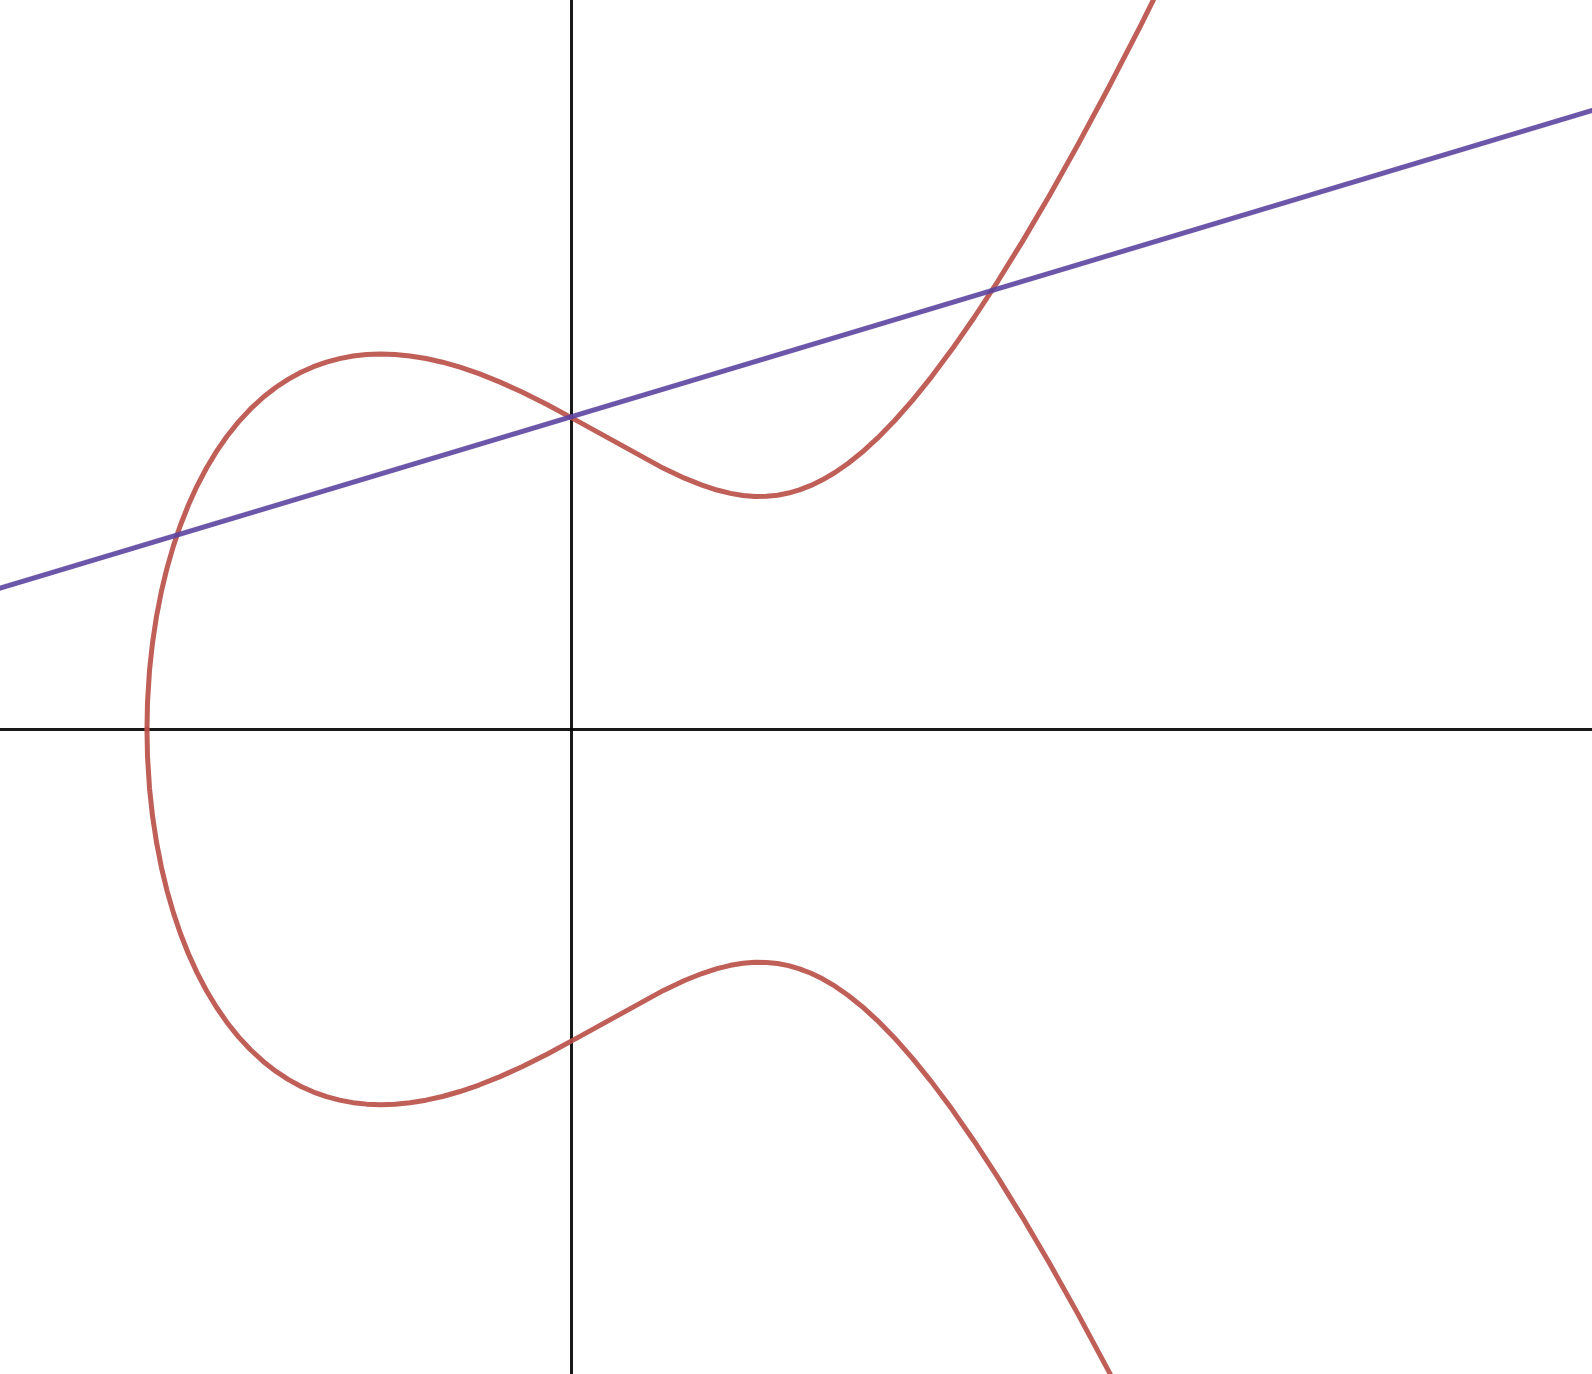
\includegraphics[width=0.5\textwidth]{images/ec_two_intersection.png}
          \end{center}
          If $P_1\neq P_2$, the slope of $L$ is
          \[\lambda = \frac{y_2-y_1}{x_2-x_1}\]
          \begin{center}
              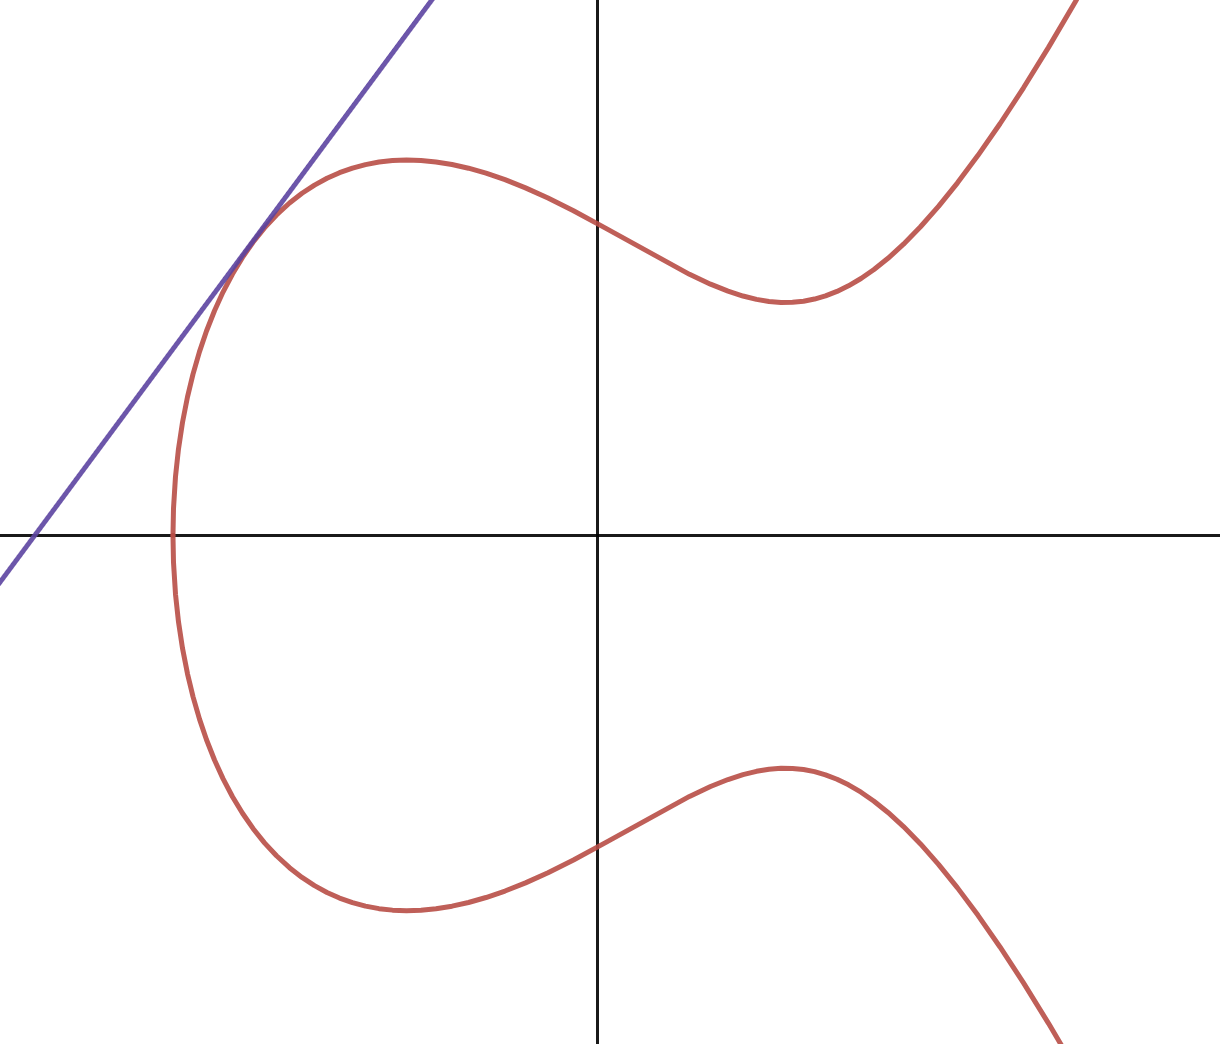
\includegraphics[width=0.5\textwidth]{images/ec_tangent.png}
          \end{center}
          If $P_1 = P_2$, then the slope would be the tangent:
          \begin{align*}
              y^2           & = x^3 + ax + b      \\
              2y\cdot dy    & = (3x^2+a)\cdot dx  \\
              \frac{dy}{dx} & = \frac{3x^2+a}{2y}
          \end{align*}
          so we have
          \[\lambda = \frac{3x^2+a}{2y}\]

          We want to solve systems
          \[\begin{cases}
                  y^2 = x^3 + ax + b \\
                  y = y_1 + \lambda(x-x_1)
              \end{cases}\]
          which gives us
          \begin{align*}
              [y_1 + \lambda(x - x_1)]^2 & = x^3 + ax + b                                       \\
              0                          & = x^3 - \boxed{\lambda^2}x^2 + (a + 2\lambda_1 x_1)x
              + b-y_1 - \lambda x_1^2                                                           \\
                                         & = (x-x_1)(x-x_2)(x-x_3)                              \\
                                         & = x^3 - \boxed{(x_1+x_2+x_3)}x^2 +
              (x_1x_3 + x_2x_3 + x_1x_2)x - x_1x_2x_3
          \end{align*}
          With some working out (taking the coefficient of $x^2$), \[\boxed{x_3 = \lambda^2 - x_1 - x_2}\] and $-y_3 = y_1 + \lambda(x_3 - x_1)$ so we have \[\boxed{y_3 = -y_1 - \lambda(x_3 - x_1)}\] are our points by addition where
          \[\lambda = \frac{y_2 - y_1}{x_2 - x_1}\]
          or when $P_1 = P_2$,
          \[\lambda = \frac{3x_1^2 + a}{2y_1}.\]
\end{itemize}

\subsection{Elliptic Curves over Finite Fields}
Our definition stays the same, except $x, y$ are elements of $\ZZ/p\ZZ$. How do we add points? We could do it geometrically, but setting this up is outside the scope of this class\dots

For addition, we use the same formulas that we've derived for $x_3$ and $y_3$, and they still make perfect sense mod $p$. \emph{For whatever reasonable notion of geometry we have over $\ZZ/p\ZZ$, they work with these formulas.}

\begin{example}
    We take elliptic curve
    \[y^2 = x^3 + x + 2\quad \text{ over }\ZZ/5\ZZ.\]
    How do we find elements in this elliptic curve? We can try them all.
    \begin{itemize}
        \item If $x = 0$, $y^2 = 2$, of which there are no solutions.
        \item If $x = 1$, $y^2 = 4$, of which $y = 2, 3$ are solutions.
        \item If $x = 2$, $y^2 = 2$ again, of which there are no solutions.
        \item If $x = 3$, $y^2 = 2$, of which there are no solutions.
        \item If $x = 4$, $y^2 = 0$, so $y = 0$ is one solution.
    \end{itemize}
    We have $(1,2), (1,3), (4,0), \cO$ are the elements of this elliptic curve. We have these
    \[\begin{array}{c|cccc}
            +     & \cO   & (1,2) & (4,0) & (1,3) \\ \hline
            \cO   & \cO   & (1,2) & (4,0) & (1,3) \\
            (1,2) & (1,2) & (4,0) & (1,3) & \cO   \\
            (4,0) & (4,0) & (1,3) & \cO   & (1,2) \\
            (1,3) & (1,3) & \cO   & (1,2) & (4,0)
        \end{array}\]
\end{example}
Let's implement this:
\begin{lstlisting}[language=Python]
O = "the point O"
def add(P1, P2, a, p):
    if P1 == O:
        return P2
    if P2 == O:
        return P1
    x1, y1 = P1
    x2, y2 = P2
    if x1 == x2 and (y1 + y2) % p == 0:
        return O
    if P1 == P2:
        lam = (3 * x1**2 + a) * ext_gcd(2 * y1, p)[0] % p
    else:
        lam = (y2 - y1) * ext_gcd(x2 - x1, p)[0] % p
    x3 = (lam**2 - x1 - x2) % p
    y3 = (lam * (x1 - x3) - y1) % p
    return x3, y3
\end{lstlisting}